
\section{Gantt Chart}

A Gantt chart was used to give a high-level overview of my project to give myself a realistic timetable of when different aspects had to be completed by. Figure~\ref{fig:gantt-chart} shows the complete version.

\newpage

\begin{landscape}
  \begin{figure}
    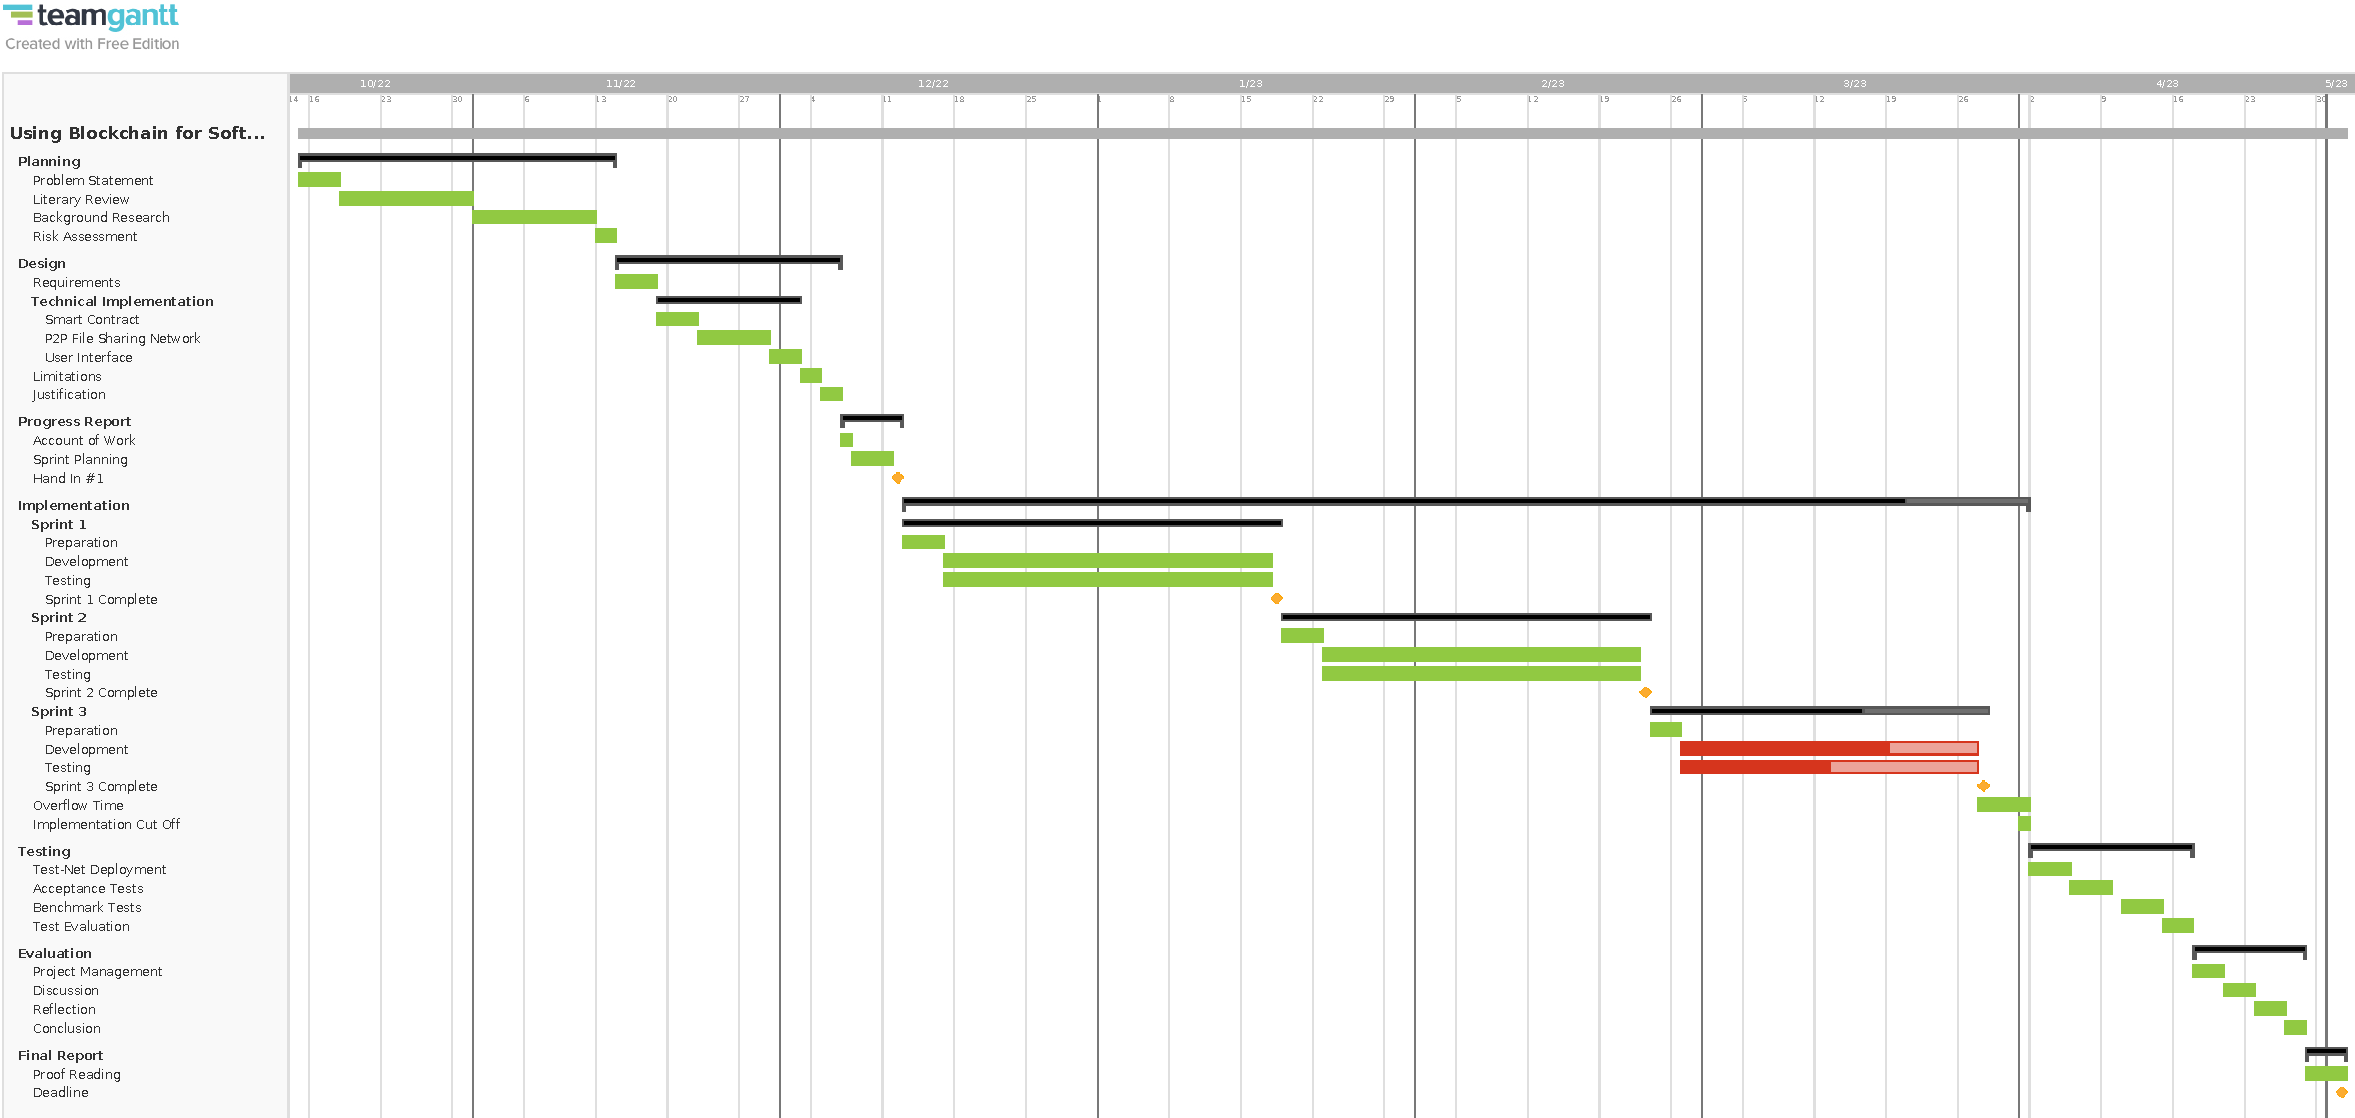
\includepdf[angle=90, scale=.95]{assets/gantt-a3-cropped.pdf}
    \vspace{150mm}
    \caption{The Gantt chart showing a breakdown of my project by task and milestones, where the red areas incidicate incomplete work. Created with TeamGantt~\cite{noauthor_free_nodate}.}
    \label{fig:gantt-chart}
  \end{figure}
\end{landscape}
